\section{Qualità di processo}
Per garantire la qualità del progetto si utilizza come riferimento lo standard ISO/IEC 12207:1995. Dopo uno studio dettagliato di tale documento sono stati scelti i processi da utilizzare e sono riportati in seguito; mentre le loro rispettive attività sono state semplificate o adattate in base alle esigenze. Questi processi fanno parte dei processi primari, di supporto ed organizzativi. \\ \\ 
In conclusione ci sono le metriche che indicano il valore accettabile e ottimale di un determinato processo preso in causa. Ogni metrica è distinta dal suo titolo rappresentativo e dal codice identificativo che è presente nella tabella sotto la sezione "Metrica". Il codice raffigura la: metrica, qualità processo 1 (mentre qualità prodotto 2), trattino separatore e numero metrica.

\subsection{Processi di sviluppo}
Sono i processi e le attività che fanno parte dello sviluppo del software e hanno lo scopo di soddisdfare tutti i requisiti concordati con il cliente.
    \subsubsection{Analisi dei requisiti}
        \paragraph{Metrica - Percentuale requisiti soddisfatti}
        È la percentuale dei requisiti che devono essere soddisfatti.

        \rowcolors{2}{grigetto}{white}
        \renewcommand{\arraystretch}{1.5}
        \begin{longtable}{ c C{4cm} c c c}
        \rowcolor{darkblue}
        \textcolor{white}{\textbf{Metrica}} & \textcolor{white}{\textbf{Nome}} & \textcolor{white}{\textbf{Sigla}} & \textcolor{white}{\textbf{Valore Accettabile}} & \textcolor{white}{\textbf{Valore Ottimale}}\\
        MQP1-01 & Percentuale Requisiti Soddisfatti & PRS & PRS=100\% & PRS=100\% \\	     
        \end{longtable}
        Formula percentuale requisiti soddisdfatti: \begin{math}{PRS = {requisiti \; soddisfatti \over requisiti \; totali}\; \cdot \; 100}\end{math}

    \subsubsection{Progettazione di dettaglio}
        \paragraph{Metrica - Incapsulamento CBO}
        Il "Coupling Between Objects" misura il numero delle classi correlate ad una classe al di fuori dalla gerarchia di ereditarietà. Più è alto il grado di coupling e più il sistema è difficile da mantenere.
        
        \rowcolors{2}{grigetto}{white}
        \renewcommand{\arraystretch}{1.5}
        \begin{longtable}{ c C{4cm} c c c}
        \rowcolor{darkblue}
        \textcolor{white}{\textbf{Metrica}} & \textcolor{white}{\textbf{Nome}} & \textcolor{white}{\textbf{Sigla}} & \textcolor{white}{\textbf{Valore Accettabile}} & \textcolor{white}{\textbf{Valore Ottimale}}\\
        MQP1-02 & Coupling Between Objects & CBO & 0$\leq$CBO$<$5 & 0$\leq$CBO$<$3 \\	     
        \end{longtable}

        \begin{itemize}
        \item N = numero classi non apparteneti alla gerarchia di ereditarietà;
        \item C = classe correlata;
        \item Formula grado di Coupling Between Objects: \begin{math}{CBO = {\sum_{i=1}^{N} \cdot \; Ci}}\end{math}.
        \end{itemize}
        
    \subsubsection{Codifica}
        \paragraph{Metrica - Livelli di profondità}
        L'applicazione per questioni di usabilità è ritenuto opportuno non integrare troppi livelli di profondità per accedere alle varie opzionalità disponibili.

        \rowcolors{2}{grigetto}{white}
        \renewcommand{\arraystretch}{1.5}
        \begin{longtable}{ c C{4cm} c c c}
        \rowcolor{darkblue}
        \textcolor{white}{\textbf{Metrica}} & \textcolor{white}{\textbf{Nome}} & \textcolor{white}{\textbf{Sigla}} & \textcolor{white}{\textbf{Valore Accettabile}} & \textcolor{white}{\textbf{Valore Ottimale}}\\
        MQP1-03 & Numero Livelli Profondità & NLP & 0$\leq$NPL$<$8 & 0$\leq$NPL$<$5 \\	     
        \end{longtable}

        \paragraph{Metrica - Numero di parametri per metodo}
        Un numero elevato di parametri per metodo può indicare il bisogno di ridurre funzionalità associate a tale metodo. Più è grande questo valore e più la possibilità aumenta nel commettere errori progettuali.
        
        \rowcolors{2}{grigetto}{white}
        \renewcommand{\arraystretch}{1.5}
        \begin{longtable}{ c C{4cm} c c c}
        \rowcolor{darkblue}
        \textcolor{white}{\textbf{Metrica}} & \textcolor{white}{\textbf{Nome}} & \textcolor{white}{\textbf{Sigla}} & \textcolor{white}{\textbf{Valore Accettabile}} & \textcolor{white}{\textbf{Valore Ottimale}}\\
        MQP1-04 & Numero di Parametri per Metodo & NPM & 0$<$NPM$<$8 & 0$<$NPM$<$4 \\	     
        \end{longtable}

        \paragraph{Metrica - Linee di codice per linee di commento}
        È il rapporto tra linee di codice e linee di commento.

        \rowcolors{2}{grigetto}{white}
        \renewcommand{\arraystretch}{1.5}
        \begin{longtable}{ c C{4cm} c c c}
        \rowcolor{darkblue}
        \textcolor{white}{\textbf{Metrica}} & \textcolor{white}{\textbf{Nome}} & \textcolor{white}{\textbf{Sigla}} & \textcolor{white}{\textbf{Valore Accettabile}} & \textcolor{white}{\textbf{Valore Ottimale}}\\
        MQP1-05 & Linee di Codice per Linee di Commento & LCLC & LCLC$\geq$0.25 & LCLC$\geq$0.30 \\	     
        \end{longtable}
        Formula valore percentuale: \begin{math}{PRS = {linee \; di \; codice \over linee \; di \; commento}}\end{math}

\subsection{Processi di supporto}
Sono i processi e le attività che aiutano gli altri processi nel raggiungimento del successo e nella qualità del progetto.
    \subsubsection{Documentazione}
        \paragraph{Metrica - Indice di Gulpease}
        È l'indice di leggibilità di un determinato testo. Calcola la lunghezza delle parole e delle frasi rispetto al numero totale delle lettere. Il valore è un intero da 0 a 100.

        \rowcolors{2}{grigetto}{white}
        \renewcommand{\arraystretch}{1.5}
        \begin{longtable}{ c C{4cm} c c c}
        \rowcolor{darkblue}
        \textcolor{white}{\textbf{Metrica}} & \textcolor{white}{\textbf{Nome}} & \textcolor{white}{\textbf{Sigla}} & \textcolor{white}{\textbf{Valore Accettabile}} & \textcolor{white}{\textbf{Valore Ottimale}}\\
        MQP1-06 & Indice di Gulpease & IG & 40$<$IG$<$100 & 80$<$IG$<$100 \\	     
        \end{longtable}
        Formula valore indice di Gulpease: \begin{math}{IG = 89 + {{300 \; \cdot \; (numero\; delle \; frasi) \; - \; 10 \; \cdot \; (numero \; delle \; lettere)}\over numero \; delle \; parole}}\end{math}
    
    \subsubsection{Garanzia di qualità}
        \paragraph{Metrica - Efficacia del processo}
        Viene indicato se il processo rispetta gli effetti e i risultati voluti. Un processo deve essere efficace\ap{G} al 100\% per garantire la sua qualità.

        \rowcolors{2}{grigetto}{white}
        \renewcommand{\arraystretch}{1.5}
        \begin{longtable}{ c C{4cm} c c c}
        \rowcolor{darkblue}
        \textcolor{white}{\textbf{Metrica}} & \textcolor{white}{\textbf{Nome}} & \textcolor{white}{\textbf{Sigla}} & \textcolor{white}{\textbf{Valore Accettabile}} & \textcolor{white}{\textbf{Valore Ottimale}}\\
        MQP1-07 & Efficacia del Processo & EP & EP=100\%  & EP=100\%  \\	     
        \end{longtable}

    \subsubsection{Verifica}
        \paragraph{Metrica - Code coverage}
        È la percentuale di copertura del codice attraversato dai test rispetto al totale del codice di base. Per dare una misurazione in termini di grandezza si adoperano le linee di codice come riferimento.
        \\ \\ %addattamento per la pagina successiva 
        \rowcolors{2}{grigetto}{white}
        \renewcommand{\arraystretch}{1.5}
        \begin{longtable}{ c C{4cm} c c c}
        \rowcolor{darkblue}
        \textcolor{white}{\textbf{Metrica}} & \textcolor{white}{\textbf{Nome}} & \textcolor{white}{\textbf{Sigla}} & \textcolor{white}{\textbf{Valore Accettabile}} & \textcolor{white}{\textbf{Valore Ottimale}}\\
        MQP1-08 & Code Coverage & CC & CC=80\%  & CC=100\%  \\	     
        \end{longtable}
        Formula valore percentuale: \begin{math}{CC = {linee \; di \; codice \; percorse \; dai  \; test \over linee \; di \; codice \; totali} \; \cdot \; 100}\end{math}

    \subsubsection{Pianificazione}
        \paragraph{Metrica - Schedule Variance}
        È il valore che indica se si è in linea (=0), in anticipo($>$0) oppure in ritardo($<$0) rispetto alla schedulazione delle attività di progetto pianificate nella baseline\ap{G}.

        \rowcolors{2}{grigetto}{white}
        \renewcommand{\arraystretch}{1.5}
        \begin{longtable}{ c C{4cm} c c c}
        \rowcolor{darkblue}
        \textcolor{white}{\textbf{Metrica}} & \textcolor{white}{\textbf{Nome}} & \textcolor{white}{\textbf{Sigla}} & \textcolor{white}{\textbf{Valore Accettabile}} & \textcolor{white}{\textbf{Valore Ottimale}}\\
        MQP1-09 & Schedule Variance & SV & SV=0  & SV$>$0  \\	     
        \end{longtable}

        \begin{itemize}
            \item VP = valore pianificato;
            \item VM = valore maturato;
            \item Formula valore di Schedule Variance: \begin{math}{SV = {VM \; - \; VP}}\end{math}.
        \end{itemize}

        \paragraph{Metrica - Budget Variance}
        È il valore che indica se la data corrente si è speso di più ($>$0) o di meno($<$0) rispetto a quanto pianificato dal budget totale.

        \begin{itemize}
            \item VP = valore pianificato;
            \item VM = valore maturato;
            \item Btot = Budget totale.
        \end{itemize}

        \rowcolors{2}{grigetto}{white}
        \renewcommand{\arraystretch}{1.5}
        \begin{longtable}{ c C{4cm} c c c}
        \rowcolor{darkblue}
        \textcolor{white}{\textbf{Metrica}} & \textcolor{white}{\textbf{Nome}} & \textcolor{white}{\textbf{Sigla}} & \textcolor{white}{\textbf{Valore Accettabile}} & \textcolor{white}{\textbf{Valore Ottimale}}\\
        MQP1-10 & Budget Variance & BV & 0$\leq$BV$<$VP  & 0$\leq$BV$\leq$Btot  \\	     
        \end{longtable}
        Formula valore di Budget Variance: \begin{math}{BV = {VM \; - \; VP}}\end{math}

\subsection{Ciclo di Deming}
    La norma ISO/IEC 12207 utilizza il ciclo di miglioramento continuo dei processi basato sulla sequenza Plan Do Check Act.

    \begin{figure}[h]
        \centering
        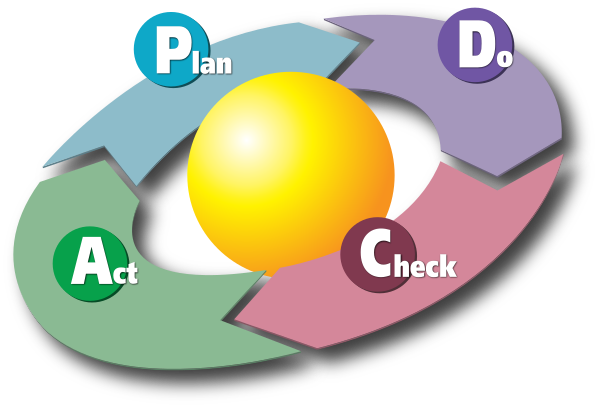
\includegraphics[scale=0.2]{sezioni/Immagini/PDCA.png}
        \caption{PCDA - Plan Do Check Act}
    \end{figure}

    \begin{itemize}
    \item \textbf{Plan}: definisce attività e scadenze necessarie al raggiungimento dei specifici obiettivi di miglioramento;
    \item \textbf{Do}: esegue le attività di "Plan";
    \item \textbf{Check}: verifica l'esito delle azioni di miglioramento rispetto alle attese. Si analizzano i risultati del "Do" e li si conforontano con gli obiettivi individuati nel "Plan";
    \item \textbf{Act}: consolida il tutto e cerca dei metodi per il prossimo miglioramento. Se il "Check" ha dimostrato che il "Plan" implementato dal "Do" è migliore rispetto ai precedenti processi standard, allora questo piano diventa il nuovo processo standard. Altrimenti il vecchio standard in uso rimarrà la baseline\ap{G}.
    \end{itemize}